\documentclass[12pt,titlepage, twoside]{article}
\usepackage[utf8]{inputenc}
\usepackage[english]{babel}
\usepackage[titletoc]{appendix}
\usepackage{graphicx}
\usepackage{lscape}
\usepackage{epstopdf}
\usepackage{wrapfig}
\usepackage{comment}
\usepackage{amsmath, amsthm, amssymb}
\usepackage{eqnarray}
\numberwithin{equation}{section}
\numberwithin{figure}{section}
\numberwithin{table}{section}
%\addcontentsline{toc}{chapter}{\listfigurename}
\usepackage{hyperref}
\usepackage{amsfonts}
\usepackage{fixltx2e}
\usepackage{nomencl}
\usepackage{natbib}
\usepackage{setspace}
\usepackage{caption}
\usepackage{subcaption}
%\usepackage[toc,page]{appendix}
\usepackage{fancyhdr}
\usepackage[top = 2cm, bottom = 2cm, outer=2 cm, inner = 3cm]{geometry}
\usepackage{footnote}
\usepackage{mathtools}
\usepackage[export]{adjustbox}

%% for including PDF pages
\usepackage{caption}
\usepackage{lipsum}
\usepackage{boxhandler}
\usepackage{pdfpages}

%% for mathematical fractals and symbosl
\usepackage{physics}

%ťhis three for degrees
\usepackage{amsmath}
\usepackage{breqn}
\usepackage{siunitx}

%% this three for numbering of footnotes
\usepackage{footmisc}
\usepackage{perpage}
\MakePerPage{footnote}

%% for using bibtex
\usepackage{natbib}
%\setcitestyle{numbers,square,sort&compress}

%\usepackage[numbers,comma,sort&compress]{natbib}
%Calls bibliography commands 
\bibliographystyle{ieeetr}


%\usepackage{blockarray}% http://ctan.org/pkg/blkarray
%\newcommand{\matindex}[1]{\mbox{\scriptsize#1}}% Matrix index


\DeclareMathOperator{\arccosh}{arccosh}
\DeclareMathOperator{\arcsinh}{arcsinh}
\DeclareMathOperator{\arctanh}{arctanh}
\DeclareMathOperator{\arctg}{arctg}
%%\captionsetup[table]{font={stretch=1.2}}     %% change 1.2 as you like
\captionsetup[figure]{font={stretch=1.5}} 

\renewcommand{\listtablename}{Seznam tabulek}
\renewcommand{\listfigurename}{Seznam obrázků}

%\usepackage{stdpage}
\let\abbrev\nomenclature
\renewcommand{\nomname}{List of Abbreviations}
\setlength{\nomlabelwidth}{.25\hsize}
\renewcommand{\nomlabel}[1]{#1 \dotfill}
\setlength{\nomitemsep}{.2cm} \makenomenclature
\newcommand{\Listofabbrev}{
\printnomenclature
\newpage
}
%%%%%%% dvakrat prelozit build.tex a pak spustit makeindex build.nlo -s nomencl.ist -o build.nls a znovu prelozit build.tex %%%%%%%-\parsep

\newcommand{\konv}[1]{\ensuremath{\stackrel{\rm #1}{\longrightarrow}}}
%\topmargin      -3cm \oddsidemargin  -1.5cm \textwidth      19cm
%\textheight     26cm

%************************************************%												%
%			Moje nastavení rozměrů				%
%												%
%************************************************
%\hoffset -1.54cm
%\voffset -0.04pt
%\evensidemargin 3 cm
%\oddsidemargin 2 cm
\topmargin -.5cm
\marginparwidth = 50pt
\marginparsep = 3pt

\textheight 217mm
%\textwidth 165mm

%\renewcommand{\baselinestretch}{1.5}

%************************************
%			REFERENCE				%
%************************************
\bibliographystyle{unsrt}


%************************************************%												%
%		Moje nastavení paragraph				%
%												%
%************************************************
% namísto subsubsubparagraph; není v obsahu, potřeba mezitím enter, jinak to nehodí číslo!

\usepackage{titlesec}

\setcounter{secnumdepth}{4}

\titleformat{\paragraph}
{\normalfont\small\bfseries}{\theparagraph}{1em}{}
\titlespacing*{\paragraph}
{0pt}{1.0ex plus 0ex minus -.5ex}{0.0ex plus 0.0ex}
%{\normalfont\normalsize\bfseries\itshape}
%***********************************
%

%************************************
%		Nedělitelná slova			%
%************************************
\hyphenation{Drucker-Prager}
\hyphenation{Mohr-Coulomb}

\newcommand\cleartooddpage{\clearpage
	\ifodd\value{page}\else\null\clearpage\fi}

\renewcommand{\footnoterule}{%
	\kern -1pt
	\hrule width \textwidth height 1pt
	\kern 2pt
}

%************************************
%			commenting todos				%
%************************************
%\usepackage[colorlinks]{hyperref}
\usepackage[colorinlistoftodos]{todonotes}
\usepackage{verbatim}




%\pagenumbering{roman} % Start roman numbering
\begin{document}




\thispagestyle{empty}
\begin{center}\setstretch{1.0}{
		{\LARGE \textsc CZECH TECHNICAL UNIVERSITY \\[0.3cm]IN PRAGUE}\\[2ex]
		{\LARGE \textsc Faculty of Civil Engineering}\\[2ex]
		{\LARGE \textsc Department of Mechanics}\\
		\vspace{1cm}
		\begin{figure}[ht!]
			\begin{center}
				{
\includegraphics[width=5cm]{lev_novy.eps}}
			\end{center}
		\end{figure}
		\vspace{1cm}
		
		{\textbf {\Huge Bachelor Thesis \\[4ex]}
			{\LARGE \bf Computational modeling of thermoset polymers with application to anchors \\[1ex]}
		}
		
		\vfill
		
		{\Large \bf Jan Vozáb }\\ [4ex]
		{\large \bf  Supervisor: Doc. Ing. Jan Vorel Ph.D.}\\[4ex]
		{\Large \bf Prague, 2018  }\\
		\newpage}
\end{center}
\thispagestyle{empty}
\begin{center}\setstretch{1.0}{
		{\LARGE \textsc \mbox{ČESKÉ VYSOKÉ UČENÍ TECHNICKÉ \\[0.3cm] V PRAZE}\\[2ex]
		{\LARGE \textsc Fakulta stavebního inženýrství}\\[2ex]
		{\LARGE \textsc Katedra mechaniky}\\
		\vspace{1cm}
	}
		\begin{figure}[ht!]
			\begin{center}
				{
\includegraphics[width=5cm]{lev_novy.eps}}
			\end{center}
		\end{figure}
		\vspace{1cm}
		
		{\textbf {\Huge Bakalářská práce \\[4ex]}
			{\LARGE \bf Počítačové modelování reaktoplastů používaných v kotevních systémech \\[1ex]}
		}
		
		\vfill
		
		{\Large \bf Jan Vozáb   }\\ [4ex]
		{\large \bf  Vedoucí práce: Doc. Ing. Jan Vorel Ph.D.}\\[4ex]
		{\Large \bf Praha, 2018  }\\
		\newpage}
\end{center}

%\pagenumbering{roman} % Start roman numbering


\setstretch{1.2}{
%\input{zadani}
\includepdf[fitpaper]{zadani.pdf}
\cleardoublepage
\newpage
\null\vfill \thispagestyle{empty}
\noindent {\bf Prohl\' a\v sen\' i:} \\
\\
\\
\\
Prohla\v suji, \v ze jsem svou bakalárskou práci vypracoval samostatn\v e a
pou\v zil jsem pouze podklady (literaturu, projekty, software, atd.) uveden\' e v
p\v rilo\v zen\' em seznamu. \\
\\
\\
\\
Nem\' am z\' ava\v zn\'y d\accent23uvod proti u\v zit\' i tohoto \v skoln\' iho d\' ila ve smyslu \S\,60
Z\' akona \v c. 121/2000 Sb., o pr\' avu autorsk\' em, o pr\' avech souvisej\' ic\' ich s
pr\' avem autorsk\' ym a o zm\v en\v e n\v ekter\' ych z\'akon\accent23u (autorsk\'y z\' akon). \\
\\
\\
\\
\\
{V Praze dne}
\\
\indent\hspace{275pt} Jan Voz\' ab
%
%
%
%
\newpage

\clearpage
%\todo[size=\tiny]{Missing abstracts}
%%%%%%%%%%%%%%%%%%%%%%%%%%%%%%%%%%%%%%%%%%%%%%%%%%%%%%%%%%%%
%% Zacatek vzorove strany %%%%%%%%%%%%%%%%%%%%%%%%%%%%%%%%%%
\thispagestyle{empty}

\noindent {\it Název práce:}\\
{\bf Počítačové modelování reaktoplastů používaných v kotevních sytémech}\\

\noindent
{\it Autor:} Jan Vozáb  \\
\\
\noindent
{\it Obor:}       Konstrukce a dopravní stavby\\
\\
\noindent
{\it Druh práce:} Bakalářská práce\\
\\
\noindent {\it Vedoucí práce:} doc. Ing. Jan Vorel, Ph.D.\\   --------------------------------------------------------------------------------------- \\

\noindent {\it Abstrakt:} 

Reaktoplasty mají v konstrukčním inženýrství důležitou roli. V porovnání s jinými odvětvími, jako je automobilový, letecký a kosmický průmysl, použité reaktoplasty nemusí být vždy v průběhu výstavby plně vytvrzené. Z tohoto důvodu může docházet ke změnám vlastností materiálu v důsledku dodatečného vytvrzování. Hlavním cílem této práce je vytvoření numerického modelu, který zachycuje dostatečně přesně vývoj materiálových vlastností a chování reaktoplastů při mechanickém zatěžování. Model v této práci je složen ze dvou částí. První je model vytvrzování, který zohledňuje vývoj materiálových parametrů v závislosti na teplotě a času. Jako druhý je použitý elasto-plastický model Drucker-Prager, který je využit na popis chování materiálu při mechanickém zatěžování.
\\
\\

\noindent {\it Klíčová slova:} dodatečné vytvrzování, reaktoplasty, Drucker-Prager, metoda konečných prvků

 \newpage
\thispagestyle{empty}
 \noindent
{\it Title:}\\
{\bf Computational modeling of thermoset polymers with application to anchors}\\

\noindent
{\it Autor:} Jan Vozáb \\
 
--------------------------------------------------------------------------------------- \\

\noindent {\it Abstract:} 

Compared to their classical appearance in the aerospace or automotive industry, in civil engineering applications they typically do not reach a fully cured state during construction. Therefore, the material may undergo post-curing causing a significant change in material parameters. The main aim of this work is to create a numerical model that describes sufficiently precisely the evolution of material properties and the behavior of thermoset polymers during mechanical loading. The model in this thesis is composed of two parts. The first is a curing model that takes into account the development of material parameters in relation to temperature and time. The second is the elasto-plastic Drucker-Prager model, which is used to describe the behavior of the material during mechanical loading.
\\
\\

\noindent 
{\it Key words:} material curing, thermosetting polymers, Drucker-Prager, finite element method
%% Konec vzorove strany %%%%%%%%%%%%%%%%%%%%%%%%%%%%%%%%%%%%
%%%%%%%%%%%%%%%%%%%%%%%%%%%%%%%%%%%%%%%%%%%%%%%%%%%%%%%%%%%%

%\end{document}

\newpage\null \vfill \noindent\thispagestyle{empty}{\bf\Large
Acknowledgment}
\bigskip


I would like to say thank to my supervisor, Doc. Ing. Jan Vorel, Ph.D., for his time, patience and for incessantly explaining the same things to me all over again. I would like to thank to my friends and classmates for their support and continuous motivation. Great thanks also belong to my family and especially my girlfriend Radka Sochorová for their psychical support for the duration of making this thesis. 

\newpage


}

\setstretch{1.35}{

\clearpage
\tableofcontents
\pagestyle{plain}
\listoffigures
\listoftables}
\newpage 

\newgeometry{top=2cm,bottom=2cm,outer=2cm,inner=3cm,includeheadfoot}

\pagestyle{fancy}
\fancyhead[RO,LE]{}
\fancyhead[RE]{\leftmark}
\fancyhead[LO]{\rightmark}
\renewcommand{\headrulewidth}{0pt}

\setstretch{1.20}{

%\pagenumbering{arabic} % Switch to normal numbers
%\setcounter{page}{1}

%\cleartooddpage
\cleardoublepage
\section*{Introduction}
\addcontentsline{toc}{section}{\protect\numberline{}Introduction}
\indent

In the last century construction engineering as well aerospace engineering  were dominated by the materials steel, aluminum, and concrete. But especially in last decade civil engineers more than ever faced often contradictory demands for designing larger, safer and more durable structures at shorter time and lower costs. This lead to improvement of old and designing of new materials. Composites are a key element of those new designs.

Composite materials often combine positive characteristic properties from more, typically two, different materials which result to better material properties. In many cases these combine a load carrying constituent, typically in the form of carbon or glass fibers, bonded to the cement or polymer based matrices. Their applications can be found in transportation as well as in civil engineering fields. In the aerospace industry we can found entire structural members made of composite materials, but in the building industry the use of polymer-based composites is limited. A typical area are members applied to existing concrete or masonry such as adhesive anchors. The commonly used polymers, typically utilized, are exothermically reacting, thermosets, e.g. epoxies or vinyl-esters. They have high filler content (including even cement and water). They have uncertain curing level and the mechanical properties due to the environmental conditions (a fully cured state is not usually reached).

Also a large range of working temperatures, which are typically expected during the lifetime leads to a post-curing and related changes in mechanical properties. These changes highly impact, in particular, structures under sustained or cyclic loads. For these challenges, the characterization of this type of materials is in high demand.  

The first chapter is focused on the description of anchors, the distribution according to the installation time and the load transfer mechanism, further failure modes of anchors are described. The second chapter is focused on thermosets, used types of polymers with anchors and overall material properties. In the third chapter models used for numerical simulation of thermoset polymers are introduced. As first of them, a non-associated Drucker-Prager model used for calculation of current stress and strain in time is explained. Then the curing model employed to calculate an evolution of material parameters is described. The fourth chapter is focused on the results and their comparison with experimental test data.


%\clearpage
%
\mbox{}
\thispagestyle{empty}
\clearpage

\section{Introduction}

In the last century construction engineering as well aerospace engineering  were dominated by the materials steel, aluminum, and concrete. But especially in last decade civil engineers more than ever faced often contradictory demands for designing larger, safer and more durable structures at shorter time and lower costs. This lead to improvement of old as designing new materials. Composites are a key element of those new designs. \todo[size=\tiny]{pokus}

Composite materials often combine positive characteristic properties from more, typically two different materials which result to better material properties. In many cases these combine a load carrying constituent typically in the form of carbon or glass fibers bonded to the cement or polymer based matrices. Their applications can be found in transportation as well in civil engineering fields. In the aerospace industry we can found entire structural members made from composite materials, but in the building industry is using of polymer-based composites limited. A typical area are members applied to existing concrete or masonry such as adhesive anchors. The commonly used polymers face challenges as:

\begin{itemize}
	\item typically utilized exothermically reacting thermosetting polymers, e.g. epoxies or vinyl-esters, with defined post-curing,
	\item high filler content, including even cement and water,
	\item uncertain curing level and the mechanical properties depending on the environmental conditions (a fully cured state is not usually reached).
\end{itemize} 

Also a large range of working temperatures, which are typically expected during the lifetime leads to post-curing and related changes in mechanical properties. These changes highly impact in particular structures under sustained or cyclic loads. For these challenges, the characterization of this type of materials is in high demand.  

\cleardoublepage
%\input{./kapitoly/kapitola20}

\cleardoublepage
%\mbox{}
%\thispagestyle{empty}

\thispagestyle{plain}
\section{Anchor systems}
Anchor is a steel element either cast into concrete or post-installed into a hardened concrete member and used to transmit applied loads, including headed bolts, hooked bolts (J- or L-bolt), headed studs, expansion anchors, or undercut anchors \cite{anchors-ACI-318M}. Anchors are typically used to connect structural elements or to fix non-structural components (or systems) to the structures. 

\begin{figure}[h!]
	\centering
	\includegraphics[width=0.9\textwidth]{obrazky/post_installed_anchor_types_repaired.png}
	\caption[Categorizing of post-installed anchors by load transfer mechanism]{Categorizing of post-installed anchors by load transfer mechanism ($R$ is direction of reaction force, $N$ is loading of anchor and $F_{exp}$ represent expansion force) \cite{hilti_anchors}: a) friction (micro-keying); b) keying (bearing/undercut); c) keying (screw-type); d) adhesion (bonding).}\label{obr:Post_installed_anchors}
\end{figure}

\subsection{Load transfer mechanisms}
In the picture \ref{obr:Post_installed_anchors} we can see different types of load transfer mechanisms. The choice of a  used mechanism affects future method of installation, resilience to different types of loading and even curing time, which some anchors need before loading. Each anchor type is described below in detail. 


\begin{itemize}
	\item \textit{Friction mechanism}
	As the name implies, the primary transfer mechanism is friction and it is results in bonding from expansion forces between the anchor and the primary structure (Fig. \ref{obr:Post_installed_anchors}a). Frictional force is proportional to the magnitude of expansion stresses generated by the anchor.The expansion is caused by a controlled torque during casting and even in some cases later to adjust for changes in the state of the base material.
	
	\item \textit{Keying mechanism}
	This transfer principle rely on the interlock of the anchor with deformations in the hole wall to resist external loading (Fig. \ref{obr:Post_installed_anchors}b,c). The bearing stresses created in the base material in the interface with the anchor bearing surface can rise to high levels due to the triaxial nature of the stress state. This type of anchors offers good resilience to variations in the base material conditions and thus represent one of the most robust solution for most anchor designs. 
	
	\item \textit{Bonding mechanism}
	This mechanism relies on adhesion between the concrete and the anchor created by adhesive (Fig. \ref{obr:Post_installed_anchors}d). The degree of bonding available is depending on the condition of the hole wall at the time of anchor installation and used type of adhesive material. This type of mechanism offers flexibility and high bod resistance for a wide variety of anchoring applications. 
\end{itemize}


x


\newpage
\subsection{Types of anchors}
\indent

Anchors can be divided by the load transfer mechanism, but another important criterion before choosing a specific solution is installation time, when is anchor fixed. As you can see in Fig. \ref{obr:Anchors}, anchors can be divided into two main groups: $\mathrm{a)}$ cast-in-place and $\mathrm{b)}$ post-installed. 


\subsubsection{Cast-in-place anchors}
The cast-in-place anchors are the simplest type of anchor. As the name suggests, these anchors are cast in the wet concrete or with reinforcement of concrete. In the Fig. \ref{obr:Anchors} we can see that most designs consist of a standard bolt with a hexagonal head (hex head bolt $\mathrm{(b.1)}$), though there are other designs such as “hooked” J bolts  $\mathrm{(b.2)}$ and L bolts $\mathrm{(b.3)}$. These anchors are very strong, and can be used in most anchor applications, but they are also difficult to cast. Therefore, they are recommended when the large embedment length or the  high tensile strength are required.

\subsubsection{Post-installed anchors}
Post-installed anchors are in general, technically sophisticated products, but are easy to install and provide more variability than cast-in anchors like headed studs. They can be cast to already complete concrete as well to masonry but they are a lot more sensitive to the boundary conditions than cast-in anchors. Most of the commercially available anchor products can be assigned to one of the major types which are categorized according to their load transfer mechanism (Fig. \ref{obr:Post_installed_anchors}).


\subsubsection{Types of post-installed anchors}
Four main groups of post-installed anchors based on load transfer mechanism and method of installation can be found in the literature.
 
	\begin{itemize}

	\item Expansion anchor. Primary principles of load transfer is friction, bearing or both. They are inserted into a drilled hole in the hardened concrete or masonry Main advantages are immediate load transfer and no temperature restrictions, but on the other hand they are not the best in transfer capacity. 

	\item Undercut anchors, which creates holding strength due to the mechanical interlock provided by undercutting the concrete near the back of the hole. This is achieved by a special tool or by the anchor itself during installation. The main load transfer method is keying. This type of anchor have benefits like high transfer capacity, immediate loading transfer, or no temperature restrictions, but they are more difficult to install. 

	\item Screw anchor is inserted into drilled hole with a diameter typically smaller than the anchor. Typical load transfer mechanism is keying. As advantages we can mention immediate full loading transfer or no temperature restrictions, but can reach just low loading capacity.

	\item Adhesive anchor is post-installed into drilled hole in hardened concrete, masonry or stone. Loads are transferred to the base material by the bond created by an adhesive on the anchor, so the load transfer mechanism is a bonding. Advantages of this type of anchor are a simple installation and a high capacity, main disadvantages are temperature restrictions and a curing time needed before loading, or the anchor would be damaged. But full curing state is not typically reached. Modeling partly cured adhesive is difficult due to a large number of variables such a loading history, time, temperature, even humidity. Modeling of this adhesive material is the main target of this thesis.
\end{itemize} 

\subsection{Loading and failure modes}
Anchor is in most cases loaded in tension and shear. This loading checks all parts of anchor, even the base material. According to a norm \cite{anchors-ACI-318M}, the strength design of anchors shall be based either on computation using design modes that satisfy requirements of the norm, or on test evaluation using the 5 percent fractile of test results for the following:

\begin{itemize}
	\item steel strength of anchor in tension,
	\item steel strength of anchor in shear, 
	\item concrete breakout strength of anchor in tension,
	\item concrete breakout strength of anchor in shear,
	\item pullout strength of anchor in tension (including adhesive), 
	\item concrete side-face blowout strength of anchor in tension,
	\item concrete pry out strength of anchor in shear.
\end{itemize} 

\begin{figure}
	\centering
	\begin{subfigure}{.5\textwidth}
		\centering
		\includegraphics[width=.9\linewidth]{obrazky/failure_models_tensile.png}
		\caption{tensile loading, where $N$ is tensile force}
		\label{obr:tensile_loaded}
	\end{subfigure}%
	\begin{subfigure}{.5\textwidth}
		\centering
		\includegraphics[width=.9\linewidth]{obrazky/failure_models_shear.png}
		\caption{shear loading, where $V$ is shear force}
		\label{obr:shear_loaded}
	\end{subfigure}
	\caption[Failure modes of anchors]{Failure modes of anchors \cite{anchors-ACI-318M}: a.1) steel failure; a.2) pullout; a.3) concrete breakout; a.4) side-face blowout; a.5) concrete splitting; b.1) steel failure preceded by concrete spall; b.2) concrete pryout for anchors far from a free edge; b.3) concrete breakout}
	\label{obr:failture_models}
\end{figure}


\begin{figure}[h!]
	\centering
	\includegraphics[width=0.6\textwidth]{obrazky/adhesive_failture_models_repaired.png}
	\caption[Failure modes of adhesive anchors in tensile]{Failure modes of adhesive anchors in tensile \cite{adhesive_anchors}: a) concrete cone failure; b) adhesive/concrete interface bond failure; c) steel/adhesive interface bond failure; d) mixed bond failure; e) bond failure; f) steel failure.}
	\label{obr:failture_adhesive_models}
\end{figure}
 
These failure modes are shown in Fig. \ref{obr:failture_models}. However, adhesive anchors have even more complicated failure modes due to full length bond, which can be damaged in different ways, see Fig. \ref{obr:failture_adhesive_models}.


\cleardoublepage
\mbox{}
\thispagestyle{empty}
\newpage
\section{Drucker-Prager model of plasticity}

\subsection{Introduction}\label{sec:drucker-prager_introduction}
\indent

Drucker-Prager model of plasticity modified Mohr-Coulomb model. Unlike Mohr-Coulomb model is Drucker-Prager model yield criterion smooth and in space of the principal stresses have form of cylindrical cone. If laboratory results are in effective rather than total stress, criterion of damage become dependent on the hydrostatic and mean stress.  

\begin{figure}[h!]
	\centering	
	\includegraphics[width=1.1\textwidth, angle=0]{obrazky/drucker-prager.png}
	\caption[Drucker-Prager a Mohr-Coulomb model $T$]{Drucker-Prager and Mohr-Coulomb yield criterion in space of principal stresses. \label{obr:F1}}
\end{figure}

\subsection{Drucker-Prager yield criterion}\label{sec:drucker-prager_yield_criterion}
\indent

Drucker-Prager model is based on the von Mises model in that the mean stress (first invariant of stress tensor) is obtained in the yield criterion equation, which has the form  

\begin{equation}\label{eq:f_yc}
	F(\sigma) = J + (\sigma_m-c)M_{JP}(\varphi) = 0,
\end{equation}

where $J$ is second invariant of stress tensor and $M_{JP}$ is used for approximation to the Mohr-Coulomb model. Is defined as

\begin{equation}\label{eq:f_Mjp}
	M_{JP} = \dfrac{\sin(\varphi)}{cos(\theta)-\frac{\sin(\theta)\sin(\varphi)}{\sqrt{3}}},
\end{equation}

\begin{equation}\label{eq:f_theta}
	\theta = \arctan{\frac{\sin{\varphi}}{\sqrt{3}}},
\end{equation}

where $\varphi$ is tangle of internal friction. Equations \ref{eq:f_Mjp} and \ref{eq:f_theta} are used to inscribe Drucker-Prager model into Mohr-Coulomb model.
Equations (\ref{eq:f_Mjp}) a (\ref{eq:f_theta}) were taken from \cite{drucker}.

\subsection{Calculation procedure and implementation}\label{sec:drucker-prager_count}
\indent

Total elastic stress can be calculated as 
\begin{equation}\label{eq:f_sigma}
	\sigma = D \varepsilon_e,
\end{equation}
where $D$ is stiffness matrix and $\varepsilon_e$ is elastic deformation. Calculation is selected as implicit, so model is implemented with increments. Then can be equation modified as
\begin{equation}\label{eq:f_sigma1}
	\sigma^{n+1} = \sigma^n+ D \mathrm{d} \varepsilon_e.
\end{equation}
Next step in calculation is find out, if is (\ref{eq:f_yc}) satisfied, shere $\sigma_m$ a $J$ is first respective second invariant of stress tensor and are defined as

\begin{equation}\label{eq:f_J}
	J = sqrt(\frac{1}{2}\sigma^TP\sigma),
\end{equation}

\begin{equation}\label{eq:f_sigM}
	\sigma_m = m^T\sigma.
\end{equation}

If is \ref{eq:f_yc} satisfied, calculation continues with next deformation increment. If no, material become to plastic flow. Because of that is defined $\mathrm{d}\lambda$, which is coefficient of plastic flow. Dependence of $J$ and $\sigma_m$ on the $\mathrm{d}\lambda$ is taken from \cite{drucker} and have form

\begin{equation}\label{eq:f_yc_lam}
F(\sigma)= \overbrace{J-\mu\mathrm{d}\lambda}^{J^{n+1}} + (\overbrace{\sigma_m-K M_{JP}(\varphi)\mathrm{d}\lambda}^{\sigma_m^{n+1}}-c)M_{JP}=0.
\end{equation}

Coefficient of plastic flow $\mathrm{d}\lambda$ is iterating with Newton-Raphson method until is (\ref{eq:f_yc_lam}) satisfied and until are increments infinitesimal. Popsána je vztahem

\begin{equation}\label{eq:f_d_lam}
\mathrm{d}\lambda^{n+1} = \mathrm{d}\lambda^n + \frac{F^n}{F'^n}.
\end{equation}

Return to the yield of plasticity is going after normal to equation (\ref{eq:f_yc}). Normal vector is counted as \cite{drucker}

\begin{equation}\label{eq:f_n}
n = \frac{\delta F}{\delta \sigma} = \frac{1}{2J}P \sigma + M_{JP}m, 
\end{equation}

and its derivation

\begin{equation}\label{eq:f_dn}
\frac{\delta n}{\delta \sigma} = \left(\frac{3}{2}\right)^{1/2} \frac{\sigma^T P \sigma P - P \sigma \sigma^T}{(\sigma^T P \sigma)^{3/2}}.
\end{equation}
\newpage
\subsection{Return to yield of plasticity}\label{sec:drucker-prager_return}
\indent

Basic equations are

\begin{equation}\label{eq:f_r}
F(\sigma)= \overbrace{J^{res}-\mu\mathrm{d}\lambda}^{J^{n+1}} + [\overbrace{\sigma_m^{res} - K M_{PP}(\varphi^{n+1})\mathrm{d}\lambda}^{\sigma_m^{n+1}}-c^{n+1}cot(\varphi^{n+1})]M_{JP}(\varphi^{n+1})=0.
\end{equation}

\begin{equation}\label{eq:C}
C_{E_d^{pl}} = c^{n+1} - c^{i-1} - h_c^n (E_d^{pl}-(E_d^{pl})^{i-1})=0
\end{equation}

\begin{equation}\label{eq:Phi}
\varTheta_{E_d^{pl}} = \varphi^{n+1} - \varphi^{i-1} - h_{\varphi}^n (E_d^{pl}-(E_d^{pl})^{i-1})=0
\end{equation}


%
%%
%%%
%%%%následuje návrat na plochu plasticity, který se provádí pomocí metody tečen (Newton-Raphsonova metoda). Ta je definována rovnicí
%%%
%%
%

\begin{comment}
Pro binární proces $a_1 a_2 \rightarrow b_1 b_2$, kde $a \neq b$ má řídící rovnice potom tvar 

\begin{equation}\label{eq:f10}
\begin{gathered}
\dfrac{dP_n}{d t} (t) = \dfrac{G}{V} \left\langle N_{a_1} \right\rangle \left\langle N_{a_2} \right\rangle \left[ P_{n-1} (t) - P_n (t) \right] \\ - \dfrac{L}{V} \left[ n^2 P_n (t) - (n+1)^2 P_{n+1} (t) \right] ,
\end{gathered}
\end{equation}
kde $G$ je $"$kreační člen$"$ definovaný vztahem $G \equiv \left\langle \sigma _G v \right\rangle $ a $L$ je $"$anihilační člen$"$ definovaný vztahem $L \equiv \left\langle \sigma _L v \right\rangle $.


Pro hmotnosti platí 

\begin{equation}\label{eq:f12}
	m_{\pi^-} = 139.570 ~\mathrm{MeV},
\end{equation}
\begin{equation}\label{eq:f14}
	m_{\pi^0} = 134.977 ~\mathrm{MeV},
\end{equation}
\begin{equation}\label{eq:f13}
	m_n = 939.565 ~\mathrm{MeV},
\end{equation}
\begin{equation}\label{eq:f15}
	m_p = 938.272 ~\mathrm{MeV},
\end{equation}
\begin{equation}\label{eq:f16}
	d_{\pi^-} = 0,
\end{equation}
\begin{equation}\label{eq:f18}
	d_{\pi^0} = 0,
\end{equation}
\begin{equation}\label{eq:f17}
	d_{n} = 2,
\end{equation}
\begin{equation}\label{eq:f19}
	d_{p} = 2 .
\end{equation}


\begin{equation}\label{eq:f20}
\sigma (\pi^+ p \rightarrow \Delta ^{++}) = \dfrac{326,5}{1 + 4\left( \dfrac{\sqrt{s} - 1,215}{0,110} \right) ^2 } \dfrac{q^3}{q^3 + (0,18)^3},
\end{equation}

kde  

\begin{equation}\label{eq:f21}
q (cm-hybnost) = \left[ \dfrac{(s - (m_{\pi} + m_p) ^2) (s - (m_{\pi} - m_p) ^2)}{4s} \right] ^{1/2} = \dfrac{m_p}{\sqrt{s}}p_{lab}.
\end{equation}

Hodnoty hmotností a spinů byly převzány z \cite{particle}.

Zároveň platí 

\begin{equation}\label{eq:f22}
\begin{gathered}
\sigma (\pi^+ p \rightarrow \Delta ^{++}) = \dfrac{3}{2} \sigma (\pi ^0 p \rightarrow \Delta^+) = 3 \sigma (\pi^- p \rightarrow \Delta^0)  \\ = \dfrac{3}{2} \sigma (\pi^0 n \rightarrow \Delta^0) = 3 \sigma (\pi ^+ n \rightarrow \Delta^+).
\end{gathered}
\end{equation}

Dále platí pro rozpadové šířky

\begin{equation}\label{eq:f23}
\dfrac{\Gamma(\Delta^+ \rightarrow \pi^+ n)}{\Gamma (\Delta ^+ \rightarrow \pi^0 n)} = \dfrac{\Gamma (\Delta^0 \rightarrow \pi ^- p)}{\Gamma (\Delta ^0 \rightarrow \pi^0 n)} = \dfrac{1}{2}.
\end{equation}

Tedy já budu potřebovat tyto dva účinné průřezy

\begin{equation}\label{eq:f24}
\sigma (\pi^- p \rightarrow \Delta^0) = \dfrac{1}{3} \sigma (\pi^+ p \rightarrow \Delta ^{++})
\end{equation}
a
\begin{equation}\label{eq:f25}
\sigma (\pi ^0 n \rightarrow \Delta ^0) = \dfrac{2}{3} \sigma (\pi^+ p \rightarrow \Delta ^{++}).
\end{equation}

\subsection{Clebsch-Gordanovy koeficienty}\label{sec:clebsch}

Izospin a jeho projekce pro jednotlivé částice

\begin{equation}\label{eq:f26}
\Delta ^0  = \left| 3/2, -1/2 \right\rangle ,
\end{equation}

\begin{equation}\label{eq:f27}
p = \left| 1/2, 1/2 \right\rangle ,
\end{equation}

\begin{equation}\label{eq:28}
n = \left| 1/2, -1/2 \right\rangle ,
\end{equation}

\begin{equation}\label{eq:29}
\pi ^0  = \left| 1, 0 \right\rangle ,
\end{equation}

\begin{equation}\label{eq:30}
\pi ^-  = \left| 1, -1 \right\rangle .
\end{equation}

Takže pro reakci $ \Delta^0 \rightarrow n + \pi^0 $ platí

\begin{equation}\label{eq:31}
\begin{gathered}
PS: \left| 1, 0 \right\rangle \left| 1/2, -1/2\right\rangle =  
\begin{bmatrix}
1       & 1/2 & 1/2 \\
0       & -1/2 & -1/2
\end{bmatrix}
\left| 1/2, -1/2 \right\rangle + 
\begin{bmatrix}
1       & 1/2 & 3/2 \\
0      & -1/2 & -1/2 
\end{bmatrix}
\left| 3/2, -1/2 \right\rangle \\ = \sqrt{\dfrac{1}{3}} \left| 1/2, -1/2 \right\rangle + \sqrt{ \dfrac{2}{3} } \left| 3/2, -1/2 \right\rangle
\end{gathered}
\end{equation}
a
\begin{equation}
LS: \left| 3/2, -1/2 \right\rangle.
\end{equation}

Pro pravděpodobnost výskytu procesu $\Delta^0 \rightarrow n + \pi^0 $ pak platí 

\begin{equation}\label{eq:32}
\left| \left\langle \Delta^0 |  n + \pi^0 \right\rangle \right|  ^2 = \left| \sqrt{\dfrac{2}{3}} \left\langle 3/2, -1/2 | 3/2, -1/2 \right\rangle \right| ^2 = \dfrac{2}{3}.
\end{equation}

Z rovnice (\ref{eq:32}) vyplývá, že účinný průřez (\ref{eq:f24}) pro reakci $p + \pi^- \rightarrow n + \pi ^0$ přenásobíme ještě koeficientem $2/3$.

Pro reakci $ \Delta^0 \rightarrow p + \pi^- $ platí

\begin{equation}\label{eq:33}
\begin{gathered}
PS: \left| 1/2, 1/2 \right\rangle \left| 1, -1 \right\rangle =  
\begin{bmatrix}
1/2      & 1 & 1/2 \\
1/2       & -1 & -1/2
\end{bmatrix}
\left| 1/2, -1/2 \right\rangle + 
\begin{bmatrix}
1/2       & 1 & 3/2 \\
1/2     & -1 & -1/2 
\end{bmatrix}
\left| 3/2, -1/2 \right\rangle \\ = - \sqrt{ \dfrac{2}{3}} \left| 1/2, -1/2 \right\rangle + \sqrt{ \dfrac{1}{3} } \left| 3/2, -1/2 \right\rangle
\end{gathered}
\end{equation}
a
\begin{equation}
LS: \left| 3/2, -1/2 \right\rangle.
\end{equation}	

Pro pravděpodobnost výskytu procesu $ \Delta^0 \rightarrow p + \pi^- $ pak platí 

\begin{equation}\label{eq:34}
\left| \left\langle \Delta^0 |  p + \pi^- \right\rangle \right|  ^2 = \left| \sqrt{\dfrac{1}{3}} \left\langle 3/2, -1/2 | 3/2, -1/2 \right\rangle \right| ^2 = \dfrac{1}{3}.
\end{equation}

Z rovnice (\ref{eq:34}) vyplývá, že účinný průřez (\ref{eq:f25}) pro reakci $n + \pi^0 \rightarrow p + \pi ^-$ přenásobíme ještě koeficientem $1/3$.

Účinné průřezy pro reakci $p + \pi^- \rightarrow \Delta ^0 \rightarrow n + \pi ^0$ mají nakonec následující tvar


\begin{equation}\label{eq:f35}
\sigma (\pi^- p \rightarrow \Delta^0) = \dfrac{1}{3} \cdot \dfrac{2}{3} \sigma (\pi^+ p \rightarrow \Delta ^{++}) = \dfrac{2}{9} \sigma (\pi^+ p \rightarrow \Delta ^{++})
\end{equation}
a
\begin{equation}\label{eq:f36}
\sigma (\pi ^0 n \rightarrow \Delta ^0) = \dfrac{2}{3} \cdot \dfrac{1}{3} \sigma (\pi^+ p \rightarrow \Delta ^{++}) = \dfrac{2}{9} \sigma (\pi^+ p \rightarrow \Delta ^{++}).
\end{equation}


Objem reakce uvažujeme $V = 125 ~\mathrm{fm^3}$.

\subsection{Chemické složení a reakce}\label{sec:chemie}
\indent

Pro potřeby průměrování přes relativní rychlosti budeme předpokládat, že jsou hybnosti rozděleny podle Boltzmannova rozdělení 

\begin{equation}\label{eq:f1}
n_i (p) \propto exp \left( - \dfrac{\sqrt{m_{i} ^{2} + p^2}}{T} \right),
\end{equation} 
kde $p$ je hybnost, $m_i$ je hmotnost částice $i$ a $T$ je teplota.

Tím vytvoříme předpoklad tepelné rovnováhy, ale chemicky budeme systém považovat v nerovnovážném stavu.

Relativní rychlost je dána vztahem 

\begin{equation}\label{eq:f2}
v_{ij} = \left[ (p_i p_j)^2 - m_i ^2 m_j ^2 \right] ^{1/2} / E_i E_j,
\end{equation}
kde $E_i$ a $E_j$ jsou energie dvou částic.

Střední hodnota součinu účinného průřezu $\sigma _{ij} ^X$ a relativní rychlosti $v_{ij}$ je definována jako

\begin{equation}\label{eq:f3}
\left\langle \sigma _{ij} ^X v_{ij} \right\rangle = \int d^3 p_i \int d^3 p_j n_i (p_i) n_j (p_j) \sigma _{ij} ^X v_{ij} ,
\end{equation}
kde $n_k (p_k)$ jsou rozdělení hybnosti částic.

Po vyintegrování rovnice (\ref{eq:f3}) získáme požadovaný vztah pro střední hodnotu součinu účinného průřezu a relativní rychlosti ve tvaru 

\begin{equation}\label{eq:f4}
\left\langle v_{ij} \sigma_{ij} ^{X} \right\rangle  = \dfrac{\int _{\sqrt{s_0}} ^{\infty} dx \sigma_{ij} ^{X} (x) K_1 (\dfrac{x}{T}) \left[ x^2 - (m_i + m_j)^2 \right] \left[ x^2 - (m_i - m_j)^2 \right] }{4 m_{i} ^{2} m_{j} ^{2} T K_2 (m_i /T) K_2 (m_j /T)},  
\end{equation}
kde $K_i$ jsou modifikované Besselovy funkce definované vztahy 

\begin{equation}\label{eq:f5}
K_1 (z) = \int _{0} ^{\infty} e ^{- z \cosh t} \cosh (t) dt,
\end{equation}

\begin{equation}\label{eq:f6}
K_2 (z) = \int _{0} ^{\infty} e ^{- z \cosh t} \cosh (2t) dt,
\end{equation}
kde $z = x/T$.

Dále  
\begin{equation}\label{eq:f7}
\sqrt{s_0} = max(m_i + m_j, \Sigma_{final} m_a)
\end{equation}
je prahová energie reakce.

Vztahy v kapitole \ref{sec:chemie} byly převzaty z \cite{ko} a \cite{tomasik}.

Prahovou energii reakce získáme z rovnice (\ref{eq:f7})
\begin{equation}\label{eq:f37}
\begin{gathered}
\sqrt{s_0} = max (m_{\pi^-} + m_p, m_{\pi ^0} + m_{n}) \\ = max(1077.8 ~\mathrm{MeV}, 1074.5 ~\mathrm{MeV}) \simeq 1.0778 ~\mathrm{GeV}.
\end{gathered}
\end{equation}

\newpage
\subsubsection{Konstantní teplota}\label{sec:konst_teplota}
\indent

Nejprve ukážeme, jak vypadají faktoriální momenty pro řídící rovnici závislou na konstantní teplotě $T$ předělené svou rovnovážnou hodnotou, abychom mohli posoudit, jak rychle termalizují.

 Pro numerické výpočty byly použity binomické počáteční podmínky s $N_0 = 0.0005$.
 
 \begin{figure}[h!]
 	\centering	
 	\includegraphics[width=1\textwidth, angle=0]{obrazky/fact_mom_T_165.png}
 	\caption[4. faktoriální moment pro různé teploty $T$]{Faktoriální momenty předělené svými rovnovážnými hodnotami pro teplotu $T = 165 ~\mathrm{MeV}$ pro 15 protonů a 10 pionů. \label{obr:F1}}
 \end{figure}
 
  \begin{figure}[h!]
  	\centering	
  	\includegraphics[width=1\textwidth, angle=0]{obrazky/fact_mom_T_165_jinak.png}
  	\caption[4. faktoriální moment pro různé teploty $T$]{Faktoriální momenty předělené svými rovnovážnými hodnotami pro teplotu $T = 165 ~\mathrm{MeV}$ pro 15 protonů a 10 pionů. \label{obr:F3}}
  \end{figure}
 
 \clearpage 
 \subsubsection{Postupná změna teploty}\label{sec:postupne}
 \indent
 
 
 Nyní necháme teplotu po úplné termalizaci faktoriálních momentů klesat podle Bjorkenova modelu z počáteční teploty $T_0 = 0.165 ~\mathrm{GeV}$ podle vztahu 
 
 \begin{equation}\label{eq:f26}
 T = T_0 \dfrac{t_0}{t}
 \end{equation}
 až na teplotu $T = 0.100 ~\mathrm{GeV}$.
 
 
 Čas $t_0$ je čas hadronizace pro teplotu $T = 0.165 ~\mathrm{GeV}$. Z Bjorkenovy závislosti teploty na čase je $t_0 = 6~\mathrm{fm/c}$.
 
  Zároveň s teplotou se mění i objem systému podle vztahu 
  
  \begin{equation}\label{eq:f38}
  V = V_0 \dfrac{t}{t_0},
  \end{equation}
  kde $V_0 = 125 ~\mathrm{fm^3}$.
  
  Pro numerické výpočty byly použity binomické počáteční podmínky s $N_0 = 0.005$.

 \begin{figure}[h!]
 	\centering	
 	\includegraphics[width=0.8\textwidth, angle=0]{obrazky/fact_moments.png}
 	\caption[Normované faktoriální momenty pro postupnou změnu teploty ze 165 MeV na 100 MeV]{Normované faktoriální momenty pro postupnou změnu teploty ze 165 MeV na 100 MeV pro čas termalizace okolo $30 ~\mathrm{fm/c}$ a pro 15 protonů a 10 pionů. \label{obr:B10}}
 	
\end{comment}

 

\cleardoublepage
%\mbox{}
%\thispagestyle{empty}
%\newpage
\section{Computational modeling}
\indent

For modeling of thermosetting polymers we have used three methods of numerical solution. Firstly, the Drucker-Prager plasticity model used to simulate the mechanical behavior. The implementation is based on the \cite{geofem} and is implemented into FEM software in C++ programming language, so it can by used for the numerical simulations of the anchors, which could be compared to real test results. Implementing into used FEM solver Mars \cite{mars} was way more complicated due to object oriented programming language. And when is the Drucker-Prager model implemented, it was proper to connect to the  curing model in Mars,already implemented, and which take into account changing of material parameters in time or temperature and hardening of the material.

\subsection{Finite element method}
\indent

Finite element method is a numerical solution used for the simulation of stresses, strains, natural frequency, heat transition, electromagnetic effects, flow of fluids, etc., on a created physical model. The main principle is the discretization of continuum to finite number of the elements, where are investigated parameters examined on a each element. FEM is used typically for inspection an already modeled structures or for determination of critical region of the structure. Through principles of this method were developed in first half of twentieths century, its massive expansion occurred with succession of a modern computer technologies due to necessary high computing power \cite{dhatt2012finite}. 
\newpage
\subsection{Vectors and matrices}
\indent

Before proceeding with the actual formulation of individual constitutive models, we first define the following matrices and vectors frequently used in this chapter:

\begin{equation}
	\boldsymbol{m} = \lbrace 1/3,1/3,1/3\rbrace ^T,
\end{equation}


\begin{equation}
	\boldsymbol{P} = \mqty[	2/3 & -1/3 & -1/3 & 0 & 0 & 0\\ 
				-1/3 & 2/3 & -1/3 & 0 & 0 & 0\\
				-1/3 & -1/3 & 2/3 & 0 & 0 & 0\\
				0 & 0 & 0 & 2 & 0 & 0\\
				0 & 0 & 0 & 0 & 2 & 0\\
				0 & 0 & 0 & 0 & 0 & 2\\],	\boldsymbol{Q} = \mqty[	1 & 0 & 0 & 0 & 0 & 0\\
				0 & 1 & 0 & 0 & 0 & 0\\
				0 & 0 & 1 & 0 & 0 & 0\\
				0 & 0 & 0 & 1/2 & 0 & 0\\
				0 & 0 & 0 & 0 & 1/2 & 0\\
				0 & 0 & 0 & 0 & 0 & 1/2\\],
\end{equation}





\subsection{Drucker-prager model of plasticity}\label{sec:drucker-prager_introduction}
\indent

If we have results of laboratory tests ploted in effective rather than total stress, then the failure criterion becomes dependent on the hydrostatic or mean stress. Then is appropriate to use Drucker-Prager yield criterion, which describes such dependence. Drucker-Prager model of plasticity is extension of the von Mises model by including mean stress (first invariant of the stress tensor) into the yield surface equation. Unlike Mohr-Coulomb model is Drucker-Prager yield criterion smooth and in space of the principal stresses have form of cylindrical cone, because of that is sometimes is Mohl-Coulomb model replaced with Drucker-Prager and as you can see in the Fig. \ref{obr:F1}. In that solution are parameters adjusted to fit or inscribe to Mohr-Coulomb model. The main advantage of that replace is about difficult return to the yield of plasticity with Mohr-Coulomb model due to its corners, which are in Drucker-Prager model excluded. Definition and calculation of Drucker-Prager model in this thesis is based on \cite{geofem}.   

\begin{figure}[h!]
	\centering	
	\includegraphics[width=0.7\textwidth, angle=0]{obrazky/drucker_prager_meridian.png}
	\caption[Drucker-Prager yield criterion on meridian plane $T$]{Drucker-Prager yield criterion in meridian plane \cite{geofem}.} \label{obr:M1}
\end{figure}

\subsubsection{Drucker-Prager yield surface}\label{sec:drucker-prager_yield_criterion}
\indent

As written above, Drucker-Prager model extend the von Mises model by including the mean stress in the yield criterion equation, which has the form  

\begin{equation}\label{eq:f_yc}
	F(\sigma) = J + (\sigma_m-c(\kappa_{1}) \cot \varphi(\kappa_{2}) )M_{JP}(\varphi(\kappa_{2})) = 0,
\end{equation}

where $J$ is a square root of the second invariant of the deviatoric stress, $\sigma_m$ is the mean stress with the form 
 
\begin{equation}\label{eq:f_J_sigM}
	J = \sqrt{\dfrac{1}{6} \left[(\sigma_{11}-\sigma_{22})^{2} + (\sigma_{11}-\sigma_{33})^{2} + (\sigma_{22}-\sigma_{33})^{2}\right] + \tau_{12}^{2} + \tau_{13}^{2}+ \tau_{23}^{2}},
\end{equation}


\begin{equation}\label{eq:f_sigM}
	\sigma_m = \dfrac{\sigma_{11} + \sigma_{22} + \sigma_{33}}{3},
\end{equation}

and $M_{JP}$ is used for approximation to the Mohr-Coulomb model and has more forms dependent on point, which approximation is needed. Three different Drucker-Prager cones are in the Fig \ref{obr:F1}. The first one, red circle, touches Mohr-Coulomb yield criterion at $\theta = 30^\circ$ (triaxial compression) with $M_{JP}$ defined as

\begin{figure}[h!]
	\centering	
	\includegraphics[width=0.8\textwidth, angle=0]{obrazky/drucker-prager_eng.png}
	\caption[Drucker-Prager a Mohr-Coulomb model $T$]{Drucker-Prager and Mohr-Coulomb yield criterion in space of principal stresses. \label{obr:F1}}
\end{figure}



\begin{equation}\label{eq:f_Mjp_30}
	M_{JP}^{\theta=30^\circ} = \dfrac{2\sqrt{3}\sin\varphi}{3-\sin \varphi},
\end{equation}

where $\varphi$ is tangle of internal friction. The second, blue circle, match Mohr-Coulomb model at  $\theta = -30^\circ$ (triaxial tension), can be obtained from

\begin{equation}\label{eq:f_Mjp_-30}
	M_{JP}^{\theta=-30^\circ} = \dfrac{2\sqrt{3}\sin\varphi}{3+\sin \varphi},
\end{equation}

and the last, the green circle is inscribed, and can be determined by

\begin{equation}\label{eq:f_Mjp_i}
	M_{JP} = \dfrac{\sin(\varphi)}{cos(\theta)-\frac{\sin(\theta)\sin(\varphi)}{\sqrt{3}}},
\end{equation}

\begin{equation}\label{eq:f_theta}
	\theta = \arctan{\frac{\sin{\varphi}}{\sqrt{3}}}
\end{equation}

In the Fig \ref{obr:M1} you can see that, Drucker-Prager model is not defined just by the yield function $F$ but also $G$, which is the plastic potential function. $G$ define vector of return to the yield of plasticity, when it is overpassed, and can be written in form 

\begin{equation}\label{eq:G}
	G = J + \left[ \sigma_m - a_{pp} \right] M_{JP}^{PP} = 0,
\end{equation}

where $a_{pp}$ follows from Fig. \ref{obr:M1}. When matching $F$ and $G$ for the current value of stress $\sigma$, result have the form

\begin{equation}\label{eq:app}
	a_{pp} = - \sigma_m^c + ( \sigma_m^c - c\cot\varphi) \dfrac{M_{JP}}{M_{JP}^{PP}}
\end{equation} 

When substituting $a_{pp}$ into the plastic potential function (\ref{eq:G}), it can be rewritten as 

\begin{equation}\label{eq:plastic_potential}
	G = J + \left[ \sigma_m - - \sigma_m + ( \sigma_m^c - c\cot\varphi) \dfrac{M_{JP}}{M_{JP}^{PP}} \right] M_{JP}^{PP} = 0,
\end{equation}

where $M_{JP}^{PP}$ is the gradient of the plastic potential function in $J-\sigma_m$ space (Fig \ref{obr:M1}). When functions of plastic potential and yield function  $M_{JP}^{PP}=M_{JP}$, model becomes associated. $M_{JP}^{PP}$  can be related to the angle of dilatation $\psi$, and can be substituted for $\varphi$ in Equations (\ref{eq:f_Mjp_-30})-(\ref{eq:f_theta}).
 
\subsubsection{Hardening and softening modulus}
\indent

In this model, inspired by the von Mises, is implemented derivation of hardening/softening modulus. To that end, we choose multi-linear form of the hardening/softening law for the cohesion $c$ and the angle of internal friction $\varphi$, as shown in Fig. \ref{obr:H}, where you can also see that, the variation of $c$ and $\varphi$ is a function of deviatoric plastic strain $E_d^{pl}$. Though the components of vector $\kappa$ may vary for each of the two strength parameters, in the present formulation is assumed a single hardening parameter

\begin{equation}\label{eq:kappa}
	\kappa = \kappa_{1} = \kappa_{2} = E_d^{pl}.
\end{equation}

\begin{figure}[h!]
	\centering	
	\includegraphics[width=0.8\textwidth, angle=0]{obrazky/hardening_softening_modulus.png}
	\caption[Hardening and softening modulus]{Hardening and softening modulus \cite{geofem}: $c_{in}$ and $c_{res}$, respective $\varphi_{in}$ and $\varphi_{res}$ represent initial and residual values of $c$ and $\varphi$.} \label{obr:H}
\end{figure}
 
Multi-linear formulation suppose that and $n^{th}$ interval in the Fig. \ref{obr:H} is active, then the current strenght parameters can be provided by

\begin{equation}\label{eq:c}
	c = c^{n-1} + h_c^n \left( E_d^{pl} -(E_d^{pl})^{n-1} \right),
\end{equation}

\begin{equation}\label{eq:phi}
\varphi = \varphi^{n-1} + h_\varphi^n\left( E_d^{pl} - (E_d^{pl})^{n-1} \right),
\end{equation}

where $h_c^n$ and $h_\varphi^n$ are the hardening/softening moduli for $c$ and $\varphi$ and can be written in the form


\begin{equation}\label{eq:h_c}
	h_c^n = \dfrac{c^n-c^{n-1}}{(E_d^{pl})^{n}-(E_d^{pl})^{n-1}}
\end{equation}

\begin{equation}\label{eq:h_phi}
 	\varphi_c^n = \dfrac{\varphi^n-\varphi^{n-1}}{(E_d^{pl})^{n}-(E_d^{pl})^{n-1}}
\end{equation}

From \cite{geofem} hardening modulus can be determined by

\begin{equation}\label{eq:H_first}
	H = \left(-\dfrac{\partial F}{\partial \kappa}\right)^T \dfrac{\partial \kappa}{\partial \lambda},
\end{equation}
\newpage
and referring to Fig. \ref{obr:H} and using Eq. (\ref{eq:H_first}) the hardening/softening modulus $H$ assumes the form 

\begin{equation}\label{eq:H}
	H = - \pdv{F}{c} \dv{c}{E_d^{pl}} \dv{E_d^{pl}}{\lambda} - \pdv{F}{\varphi} \dv{\varphi}{E_d^{pl}} \dv{E_d^{pl}}{\lambda},
\end{equation}

where
\begin{align}
\pdv{F}{\varphi}& = \dfrac{c}{\sin^2\varphi} M_{JP} + (\sigma_m - c\cot \varphi) \dv{M_{JP}}{\varphi},\label{eq:F/phi}\\
\dv{F}{c}& = - \cot \varphi M_{JP},\\
\dv{c}{\kappa}& = \dv{c}{E_d^{pl}} = h_c,\\
\dv{\varphi}{\kappa}& = \dv{\varphi}{E_d^{pl}} = h_\varphi
\end{align}

Partial derivations of $M_{JP}$ with respect to $\varphi$ for selected values of $\theta$ are

\begin{align}
	\dv{M_{JP}^{ins}}{\varphi}					& = \dfrac{3\sqrt{3}\cos \varphi}{(3 + \sin^2 \varphi)^{\frac{3}{2}}},\\
	\dv{M_{JP}^{\theta = \ang{-30}}}{\varphi}	& = \dfrac{6\sqrt{3}\cos \varphi}{(1-\sin \varphi)^2},\\
	\dv{M_{JP}^{\theta = \ang{30}}}{\varphi}	& = \dfrac{6\sqrt{3}\cos \varphi}{(1+\sin \varphi)^2}.
\end{align}


When we accept the strain hardening approach, then we can write

\begin{align}
	\dd\varepsilon^{pl}& = \dd\lambda\pdv{G}{\sigma} = \dd\lambda\dfrac{1}{2J}P\sigma,\\
	\dd\kappa& = \dd E_d^{pl} = \sqrt{2(\varepsilon^{pl})^T \text{\textbf{QPQ}} \varepsilon^{pl} } = \dd \lambda = \dv{E_d^{pl}}{\lambda} = 1.\label{eq:dkappa}
\end{align}

With final substitution of Eq. (\ref{eq:F/phi})-(\ref{eq:dkappa}) back into Eq. (\ref{eq:H}), result is searched form of the hardening/softening modulus as

\begin{equation}\label{eq:H_final}
	H = h_c \cot\varphi M_{JP} - h_\varphi \left[ \dfrac{c}{\sin^2 \varphi} M_{JP} + (\sigma_m - c \cot \varphi) \dv{M_{JP}}{\varphi} \right].
\end{equation}


\subsubsection{Calculation procedure and implementation}\label{sec:drucker-prager_count}
\indent

Total elastic stress can be calculated as 
\begin{equation}\label{eq:f_sigma}
\sigma = \text{\textbf{D}}^{el} \varepsilon_{el},
\end{equation}
where \textbf{D}$^{el}$ is ordinary stiffness matrix and $\varepsilon_e$ is elastic deformation. Calculation is performed in  implicit software \cite{mars}, so model is implemented with increments. Then can be equation modified as

\begin{equation}\label{eq:f_sigma1}
	\sigma^{n+1} = \sigma^n+ \text{\textbf{D}}^{el} \mathrm{d} \varepsilon_{el}.
\end{equation}

Next step in calculation is determine, if is Eq. (\ref{eq:f_yc}) satisfied, if is, strains ans stresses are stored, and calculation continues with next deformation increment. If yield function exceeded, material behavior become to be from basic elastic to elasto-plastic with hardening. Due to higher amount of the variables, which describe return to the yield of plasticity, is necessary to implement the Jacobian matrix\footnote{Matrix of partial derivations}. There are four material parameters that may be calculated, when is performed return to yield of plasticity:

\begin{itemize}
	\item $\Delta\lambda$ - Coefficient of plastic flow,
	\item $c$ - Cohesion,
	\item  $\varphi$ - Angle of friction,
	\item $\psi$ - Angle of dilatation.
\end{itemize}

Before of describing Jacobian matrix, we need to find out basic equations, which are used in it and define dependence of all variables. 
Plastic strain increment have the form 

\begin{equation}
	\dd \varepsilon^{pl} = \Delta \lambda \pdv{G}{\sigma},
\end{equation}

and with accepting this flow rule, increments of yield respective plastic strain have the form 

\begin{align}
	\dd \varepsilon_\nu^{pl} &= \dd \lambda \pdv{G}{\sigma_m} = \Delta \lambda M_{JP}^{PP} \sin \psi,\\
	%\dd e^{pl} &= \dd \lambda \pdv{G}{s} = \dd \lambda \dfrac{\text{\textbf{G}}^{-1}s}{2J}\text{ where } s = \text{\textbf{PQ}}\sigma,\\
	\dd E_{d}^{pl} &= \dd \lambda \pdv{G}{J} = \Delta \lambda,
\end{align}

which further allows writing the corresponding stresses at the end of the $i+1$ load increment as  

\begin{align}
	\sigma_m^{i+1} &= \sigma_m^{tr} - K M_{JP}^{PP} (\sin \psi^{i+1}) \Delta \lambda,\\
	%s^{i+1} &= s^{tr} - 2\mu \Delta \lambda\dfrac{s^{i+1}}{2J^{i+1}} = \dfrac{s^{tr}}{1 + \dfrac{\mu \Delta \lambda}{J^{i+1}}} = s^{tr} \left( 1 - \dfrac{\mu \Delta \lambda}{J^{tr}}   \right),\\
	J^{i+1} &= J^{tr} + \mu \Delta \lambda,
\end{align}

where $K$ is the bulk modulus and $\mu$ represent the elastic shear modulus to avoid misinterpretation with the plastic potential function. Now can be the Jacobian matrix defined.

\begin{itemize}
	\item Primary variables
	
	\begin{equation}
		\lbrace \mathbf{a} \rbrace ^T = \lbrace \Delta \lambda, c^{i+1}, \varphi^{i+1}, \psi^{i+1} \rbrace.
	\end{equation}
	
	\item Residuals
	\begin{equation}
		\lbrace \mathcal{r} \rbrace =  \lbrace \mathcal{F}, \mathcal{C}, \mathrm{\Phi}, \mathrm{\Psi} \rbrace,
	\end{equation}
	where \begin{align}
		\mathcal{F} &= \overbrace{J^{tr}-\mu\Delta\lambda}^{J^{i+1}} + [\overbrace{\sigma_m^{tr}-K M_{JP}^{PP}(\sin \psi^{i+1})\Delta\lambda}^{\sigma_m^{i+1}}-c^{i+1}\cot\varphi^{i+1}]M_{JP}(\sin\varphi^{i+1}),\label{eq:f_yc_lam}\\
		\mathcal{C} &= c^{i+1} - \hat{c} = 0,\label{eq:C_jac}\\
		\mathrm{\Phi} &= \varphi^{i+1} - \hat{\varphi} = 0,\label{eq:phi_jac}\\
		\mathrm{\Psi} &= \psi^{i+1} - \hat{\psi} = 0.
	\end{align}
	Variables $\hat{c}$ and $\hat{\varphi}$ follows Eq.(\ref{eq:c}) and (\ref{eq:phi}) and the current value of dilatation angle $\hat{\psi}$ can be, with help of Rowe's dilatation theory in triaxial compression, written as
	\begin{equation}
		\sin \hat{\psi} = \dfrac{\sin \varphi^{i+1} - \sin \varphi_{cv}}{1_- \sin \varphi^{i+1} \sin \varphi_{cv}},
	\end{equation}
	where $\varphi_{cv}$ is constant-volume friction angle.
	
	\item Local Newton-Raphson method
	\begin{equation}\label{eq:newton_raphson}
		\lbrace a^{i+1} \rbrace _{k+1} = \lbrace a^{i+1}_k \rbrace - [\text{\textbf{H}}]^{-1} \lbrace r \rbrace_k 
	\end{equation}
	
	\item Jacobian matrix $[\textbf{H}]$
	\begin{equation}
		[\text{\textbf{H}}] = \mqty[\pdv{J}{\Delta \lambda} \pdv{\mathcal{F}}{\sigma_m} \pdv{\sigma_m}{\Delta \lambda} & \pdv{\mathcal{F}}{c} & \pdv{\mathcal{F}}{\varphi} + \pdv{\mathcal{F}}{M_{JP}} \pdv{M_{JP}}{\sin \varphi} & \pdv{\mathcal{F}}{M_{JP}^{PP}} \pdv{M_{JP}^{PP}}{\sin \psi}\\
		\pdv{\mathcal{C}}{\hat{c}} = \pdv{\hat{c}}{\Delta \lambda} & \pdv{\mathcal{C}}{c} & 0 & 0\\
		\pdv{\mathrm{\Phi}}{\sin \hat{\varphi}} = \pdv{\hat{\varphi}}{\Delta \lambda} & 0 & \pdv{\mathrm{\Phi}}{\sin \varphi} & 0 \\
		0 & 0 & \pdv{\mathrm{\Psi}}{\sin \hat{\psi}} \pdv{\sin \hat{\psi}}{\sin \varphi} & \pdv{\mathrm{\Psi}}{\sin \psi}]
	\end{equation}
	where partial derivations are
	
	\begin{align}
		&\pdv{J}{\Delta \lambda} \pdv{\mathcal{F}}{\sigma_m} \pdv{\sigma_m}{\Delta \lambda}  = -\mu - K M_{JP}^{PP}M_{JP},\\
		&\pdv{\mathcal{F}}{c} = -M_{JP}\tan\varphi,\\
		&\pdv{\mathcal{F}}{\varphi} + \pdv{\mathcal{F}}{M_{JP}} \pdv{M_{JP}}{\sin \varphi} = M_{JP} \dfrac{c}{\sin^2\varphi \cos\varphi} + \left( \sigma_m \dfrac{c}{\tan \varphi} \right) \dv{M_{JP}}{\sin \varphi}, \\
		&\pdv{\mathcal{F}}{M_{JP}^{PP}} \pdv{M_{JP}^{PP}}{\sin \psi} = -K \Delta \lambda \dv{M_{JP}^{PP}}{\sin \psi},\\
		&\pdv{\mathcal{C}}{\hat{c}} = \pdv{\hat{c}}{\Delta \lambda} = -h_c, \\
		&\pdv{\mathcal{C}}{c} = 1,\\
		&\pdv{\mathrm{\Phi}}{\sin \hat{\varphi}} = \pdv{\hat{\varphi}}{\Delta \lambda} = -\cos(\varphi) h_{\varphi},\\
		&\pdv{\mathrm{\Phi}}{\sin \varphi} = 1,\\
		&\pdv{\mathrm{\Psi}}{\sin \hat{\psi}} \pdv{\sin \hat{\psi}}{\sin \varphi} = -\dfrac{1 - \sin^2\varphi_{cv} }{1-\sin \varphi \sin \varphi_{cv}},\\
		&\pdv{\mathrm{\Psi}}{\sin \psi} = 1.
	\end{align}
	
	Derivation of $M_{JP}$ with respect to $\sin \varphi$ is not writed in exact form due to variable equation of $M_{JP}$ (\ref{eq:f_Mjp_30})-(\ref{eq:f_Mjp_i}).
	
	\item Initial conditions
	
	\begin{align}
		\lbrace a_0 \rbrace^T &= \lbrace 0, c^i, \sin \varphi^i, \sin \psi^i \rbrace,\\
		\lbrace r_0 \rbrace^T &= \lbrace J^{tr} + (\sigma_m^{tr}-c^i\cot\varphi^i)M_{JP}(\sin\varphi^i), 0, 0, 0 \rbrace.
	\end{align}
	
\end{itemize} 

\subsubsection{Apex problem}
\indent

In the Fig \ref{obr:apex_cones} you can see two cones. First $K_\varepsilon$ (following direction of the plastic strain vector), which shows inadmissible region for the plastic strain increment, and $K_\sigma$, which show the admissible stress domain. Its obvious that, if is standard stress point in region $K_\sigma$, material behaviors is elastic, when it is outside of $K_\sigma$ but also outside of $K_\varepsilon$, computation is performing regular stress return. But the non-associated flow rule restrict the plastic strain increment to belong in the cone $K_\varepsilon$ (Eq. \ref{eq:eps_apex}), so if it belongs, stress should be returned to the apex point. That situation may occur in two cases (Fig. \ref{obr:apex_return}): $(a)$ right after load increment, bud also $(b)$, when performing regular stress return, due change of material parameters. Such a situation can be referred as an "apex problem". 

\begin{equation}\label{eq:eps_apex}
	\dot{\varepsilon}_v \geq M_{JP}^{PP} \dot{E}_d^{pl}.
\end{equation}

In the literature we can find two different stands for performing apex problem:

\begin{itemize}
	\item Return with constant material parameters.
	\item Return with hardening/softening material.
\end{itemize}
At the first case, stress point just return to the apex (Fig.\ref{obr:apex_cones}), so stress form is

\begin{equation}\label{eq:sigPL}
	\sigma^{i+1} = 3c^{i} \cot \varphi^{i} \textbf{m}.
\end{equation}

In \cite{geofem} author show a variational form of the flow rule to show through the concept of bi-potentials that the vector of plastic strain increments for the apex problem is provided by

\begin{equation}\label{eq:epsPL}
	\Delta\varepsilon^{pl} = (\textbf{D})^{-1}( \sigma^{tr} - 3 c^{i+1} \cot \varphi^{i+1} \textbf{m} )
\end{equation}

under condition



\begin{equation}\label{eq:flow_condition}
\dfrac{1}{G} M_{JP}^{PP} J^{tr} - \dfrac{1}{K} (\sigma_m^{tr} - c^i \cot \varphi^i) < 0.
\end{equation}

Note that Eq. (\ref{eq:flow_condition}) is essentially linearized from of a Eq. (\ref{eq:sigPL}).

\begin{figure}[h!]
	\centering	
	\includegraphics[width=0.8\textwidth, angle=0]{obrazky/apex_cones.png}
	\caption[Apex abmissible regions]{Apex admissible regions for stresses and plastic strain rates \cite{geofem}.} \label{obr:apex_cones}
\end{figure}


\begin{figure}[h!]
	\centering	
	\includegraphics[width=0.8\textwidth, angle=0]{obrazky/apex_recursive_return.png}
	\caption[Apex return]{Apex regular and singular return \cite{geofem}: .} \label{obr:apex_return}
\end{figure}


If we choose second approach of assuming hardening/softening material, we need to update $c$ and $\varphi$ with apex return. Procedure is similar to the regular plasticity return, but with different equations. Before proceeding, we recall that the strain hardening hypotheses is adopted with a single hardening/softening parameter $\kappa$ with form

\begin{equation}\label{eq:hardening_parameter}
	\dot{\kappa} = \dot{E}_d^{pl}
\end{equation}

With Eq. \ref{eq:hardening_parameter} we can reach incremental nonlinear equation with form

\begin{equation}
	\mathcal{E} = \Delta E_d^{pl} - \overbrace{\sqrt{2(\Delta \varepsilon^{pl})^T \textbf{QPQ}\Delta\varepsilon^{pl}} }^{\Delta \hat{E}_d^{pl}}=0
\end{equation}

which would be solved simultaneously with Eq.(\ref{eq:C_jac}) and (\ref{eq:phi_jac}). Note that the increment of plastic strain given by Eq. (\ref{eq:epsPL}) is a function of current strength parameters

\begin{equation}
	\Delta\varepsilon^{pl} = \Delta\varepsilon^{pl} (c^{i+1}, \varphi^{i+1}).
\end{equation}

Due to analogy with the regular return to the yield surface we can also use Newton-Raphson method (Eq.(\ref{eq:newton_raphson})). The calculation procedure is defined:

\begin{itemize}
	\item Primary variables
	
	\begin{equation}
		\lbrace a \rbrace^T = \lbrace \Delta E_d^{pl}, c^{i+1}, \varphi^{i+1} \rbrace.
	\end{equation}
	
	\item Residuals
	
	\begin{equation}
		\lbrace r \rbrace ^T = \lbrace \mathcal{E}, \mathcal{C}, \mathrm{\Phi} \rbrace
	\end{equation}
	
	\item Jacobian Matrix [\textbf{H}]
	
	\begin{equation}
		[\text{\textbf{H}}] = \mqty[\pdv{\mathcal{E}}{\Delta E_d^{pl}} & \pdv{\mathcal{E}}{\Delta\varepsilon^{pl}}^T \pdv{\Delta\varepsilon^{pl}}{c} & \pdv{\mathcal{E}}{\Delta\varepsilon^{pl}}^T \pdv{\Delta\varepsilon^{pl}}{\sin \varphi}\\
		\pdv{\mathcal{C}}{\Delta E_d^{pl}} = \pdv{\mathcal{C}}{\Delta \lambda} & \pdv{\mathcal{C}}{c} & 0 \\
		\pdv{\mathrm{\Phi}}{\Delta E_d^{pl}} = \pdv{\mathrm{\Phi}}{\Delta \lambda} & 0 & \pdv{\mathrm{\Phi}}{\sin \varphi}]
	\end{equation}
	\newpage
	where partial derivations have the form\
	
	\begin{align}
		&\pdv{\mathcal{E}}{\Delta E_d^{pl}} = 1,\\
		&\pdv{\mathcal{E}}{\Delta\varepsilon^{pl}}^T \pdv{\Delta\varepsilon^{pl}}{c} =  -\dfrac{2}{\Delta E_d^{pl}} \Delta e_{pl}^T (-3\cos\varphi^{i+1}\textbf{m}) = \dfrac{6\cos\varphi^{i+1}}{ \Delta E_d^{pl}} \Delta e_{pl}^T \textbf{m},\\
		&\pdv{\mathcal{E}}{\Delta\varepsilon^{pl}}^T \pdv{\Delta\varepsilon^{pl}}{\sin \varphi} = \pdv{\Delta\varepsilon^{pl}}{c} =  -\dfrac{2}{ \Delta E_d^{pl}} \Delta e_{pl}^T (-3c^{i+1}\textbf{m}) = \dfrac{6 c^{i+1}}{ 
		 \Delta	E_d^{pl}} \Delta e_{pl}^T \textbf{m} ,\\
		&\pdv{\mathcal{C}}{\Delta E_d^{pl}} = \pdv{\mathcal{C}}{\Delta \lambda} =  -h_c,\\
		&\pdv{\mathcal{C}}{c} = 1,\\
		&\pdv{\mathrm{\Phi}}{\Delta E_d^{pl}} = \pdv{\mathrm{\Phi}}{\Delta \lambda} = -\cos(\varphi) h_{\varphi} ,\\
		&\pdv{\mathrm{\Phi}}{\sin \varphi} = 1.
	\end{align}
	
	where $e_{pl}$ is deviatoric part of plastic strain tensor. 
		
	\item Initial conditions
	\begin{equation}
		\lbrace a_0 \rbrace^T = \lbrace 0, c^i, \varphi^i\rbrace,
	\end{equation}
	
	\begin{equation}
		\lbrace r_0 \rbrace^T = \lbrace \sqrt{2(\Delta \varepsilon^{pl})^T(c^i, \varphi^i) \textbf{QPQ}\Delta\varepsilon^{pl}(c^i, \varphi^i)}, 0, 0\rbrace.
	\end{equation}
\end{itemize}
 


\cleardoublepage
\thispagestyle{plain}
\section{Results}
\indent

Both implemented models in Mars solver \cite{mars} were tested for the accuracy of the results with real data. 

\subsection{Testing of Drucker-Prager model}
\indent
 
For testing accuracy of implemented Drucker-Prager model we choose experimental test taken from \cite{Deuch_phd_thesis}, where we can find compression test of the polymer mortar. As you can see in the Fig. \ref{obr:test_param}, it is a classic compression test, when is examined element compressed with testing equipment. Specific parameters of the tested element and equipment you can find in the Fig. \ref{obr:test_param}. As you can se in the Fig. \ref{obr:Compresion_test}, apparature is in the modeled object simplified to the two plates that are perpendicular to each other. In the model is the test specimen completely fixed to the bottom plate, but the top plate affect the sample with a friction force, so it can move on the plate, and also the plate can rotate.


\begin{figure}[h!]
	\centering
	\includegraphics[width=0.8\textwidth]{obrazky/test_parameters.png}
	\caption[Compression test parameters]{Compression test parameters \cite{Deuch_phd_thesis}: a) dimensions of the apparature; b) parameters of the specimen.}\label{obr:test_param}
\end{figure}

\begin{figure}[h!]
	\centering
	\includegraphics[width=0.6\textwidth]{obrazky/Compresion_test_3d.png}
	\caption[Compression test sample]{Compression test sample: on the surface you can see computed magnitude of displacement of the Drucker-Prager model without hardening of parameters.}\label{obr:Compresion_test}
\end{figure}

In the Fig \ref{obr:Compresion_test} you can see a slightly rotated deformation from the Z axis, which is caused the displacement of the sample from the top plate and its rotation. 

\begin{figure}[h!]
	\centering
	\includegraphics[width=1\textwidth]{obrazky/compression_test.eps}
	\caption[Compresion tests]{Compression tests compared to the real specimen result \cite{Deuch_phd_thesis}}\label{obr:Compresion_2d}
\end{figure}


The most important graph, where we can compare model accuracy to the real behavior is the Fig \ref{obr:Compresion_2d}. First line are experimental data taken from \cite{Deuch_phd_thesis}, other are results from test of the Drucker-Prager model. Red line represent Drucker-Prager model, where $M_{JP}$ is computed with Eq. (\ref{eq:f_Mjp_30}), second blue with Eq. (\ref{eq:f_Mjp_-30}) and the last, orange is computed with Eq. (\ref{eq:f_Mjp_i}). This three computations have constant cohesion $c$ and angle of friction $\varphi$. Fourth line is model with hardening of cohesion $c$, which have constant value of $20~\mathrm{MPa}$, until deviatoric plastic strain $E_d^{pl}$ increase from the value $0,05$. The second change, where cohesion become again constant with value $40~\mathrm{MPa}$, will happen when $E_d^{pl}$ reach value of $0,05$. The range between this two changes of $E_d^{pl}$ is hardening of the material. The last model is similar to the fourth with difference of cohesion parameters, which are constant from the start with value of $15~\mathrm{MPa}$ and increase to $60~\mathrm{MPa}$, when $E_d^{pl}$ reach value of $0,15$. 

In the Graph we can see that Drucker-Prager model without hardening simulate behavior with the least precision. Beginning of the computation is similar, but then real specimen started to increase deformation with higher speed. The fourth model is more precise than models without hardening, as it approaches direction of deformation increasing with the real test. But it have too much strength, which is greatly inaccurate. The last model mimics the behavior of the material most of all the simulations performed, which shows that variability of hardening/softening of the material parameters can help model to be more precise. But used approach with changing only cohesion $c$ parameter can be slightly inaccurate in high deformations of the material. This can be improved to the future with changing of angle of friction $\varphi$ and higher amount of intervals, which could more approximate real material behavior. Another solution, which can be done to the future is implementing of the Cap model to the Drucker-Prager, which is compression strength limit of the material. This has the effect to the yield of plasticity, which, when subjected to high compressive stress, turns to the axis volumetric stress. 



\begin{figure}[h!]
	\centering
	\includegraphics[width=0.6\textwidth]{obrazky/compression_zpevneni_parametry.png}
	\caption[Types of anchors]{Types of anchors ($h_{ef}$ is effective anchor length) \cite{anchors-ACI-318M}: a) cast-in-place; b) post-installed.}\label{obr:Compresion_parameters}
\end{figure}

All next Figs. of Drucker-Prager compresion test \ref{obr:Compresion_parameters}, \ref{obr:Compresion_plastic_srain} and \ref{obr:Compresion_total_strain} are from the model with hardening of cohesion $c$. In the Fig \ref{obr:Compresion_parameters} you can see that the angle of friction is constant, but cohesion is changing with increasing of deviatoric plastic strain. When we compare Figs \ref{obr:Compresion_plastic_srain} and \ref{obr:Compresion_total_strain}, we can see that distribution of the strain is similar.



\begin{figure}[h!]
	\centering
	\includegraphics[width=0.7\textwidth]{obrazky/compression_zpevneni_pl_strain.png}
	\caption[Types of anchors]{Types of anchors ($h_{ef}$ is effective anchor length) \cite{anchors-ACI-318M}: a) cast-in-place; b) post-installed.}\label{obr:Compresion_plastic_srain}
\end{figure}


\begin{figure}[h!]
	\centering
	\includegraphics[width=0.9\textwidth]{obrazky/compression_zpevneni_strain.png}
	\caption[Types of anchors]{Types of anchors ($h_{ef}$ is effective anchor length) \cite{anchors-ACI-318M}: a) cast-in-place; b) post-installed.}\label{obr:Compresion_total_strain}
\end{figure}

\subsection{Results of curing model}
\indent

Curing model were already implemented into Mars FEM solver, but when we want to use it, we need to compare results of the computation with article, where was model presented \cite{heinrich2012generation}. In the Fig. \ref{obr:Curing_cube} we can see that the curing is distributed with most cured material in the center of the cube and 


\begin{figure}[h!]
	\centering
	\includegraphics[width=0.9\textwidth]{obrazky/curing__and_temperature.png}
	\caption[Types of anchors]{Types of anchors ($h_{ef}$ is effective anchor length) \cite{anchors-ACI-318M}: a) cast-in-place; b) post-installed.}\label{obr:Curing_cube}
\end{figure}



\begin{figure}[h!]
	\centering
	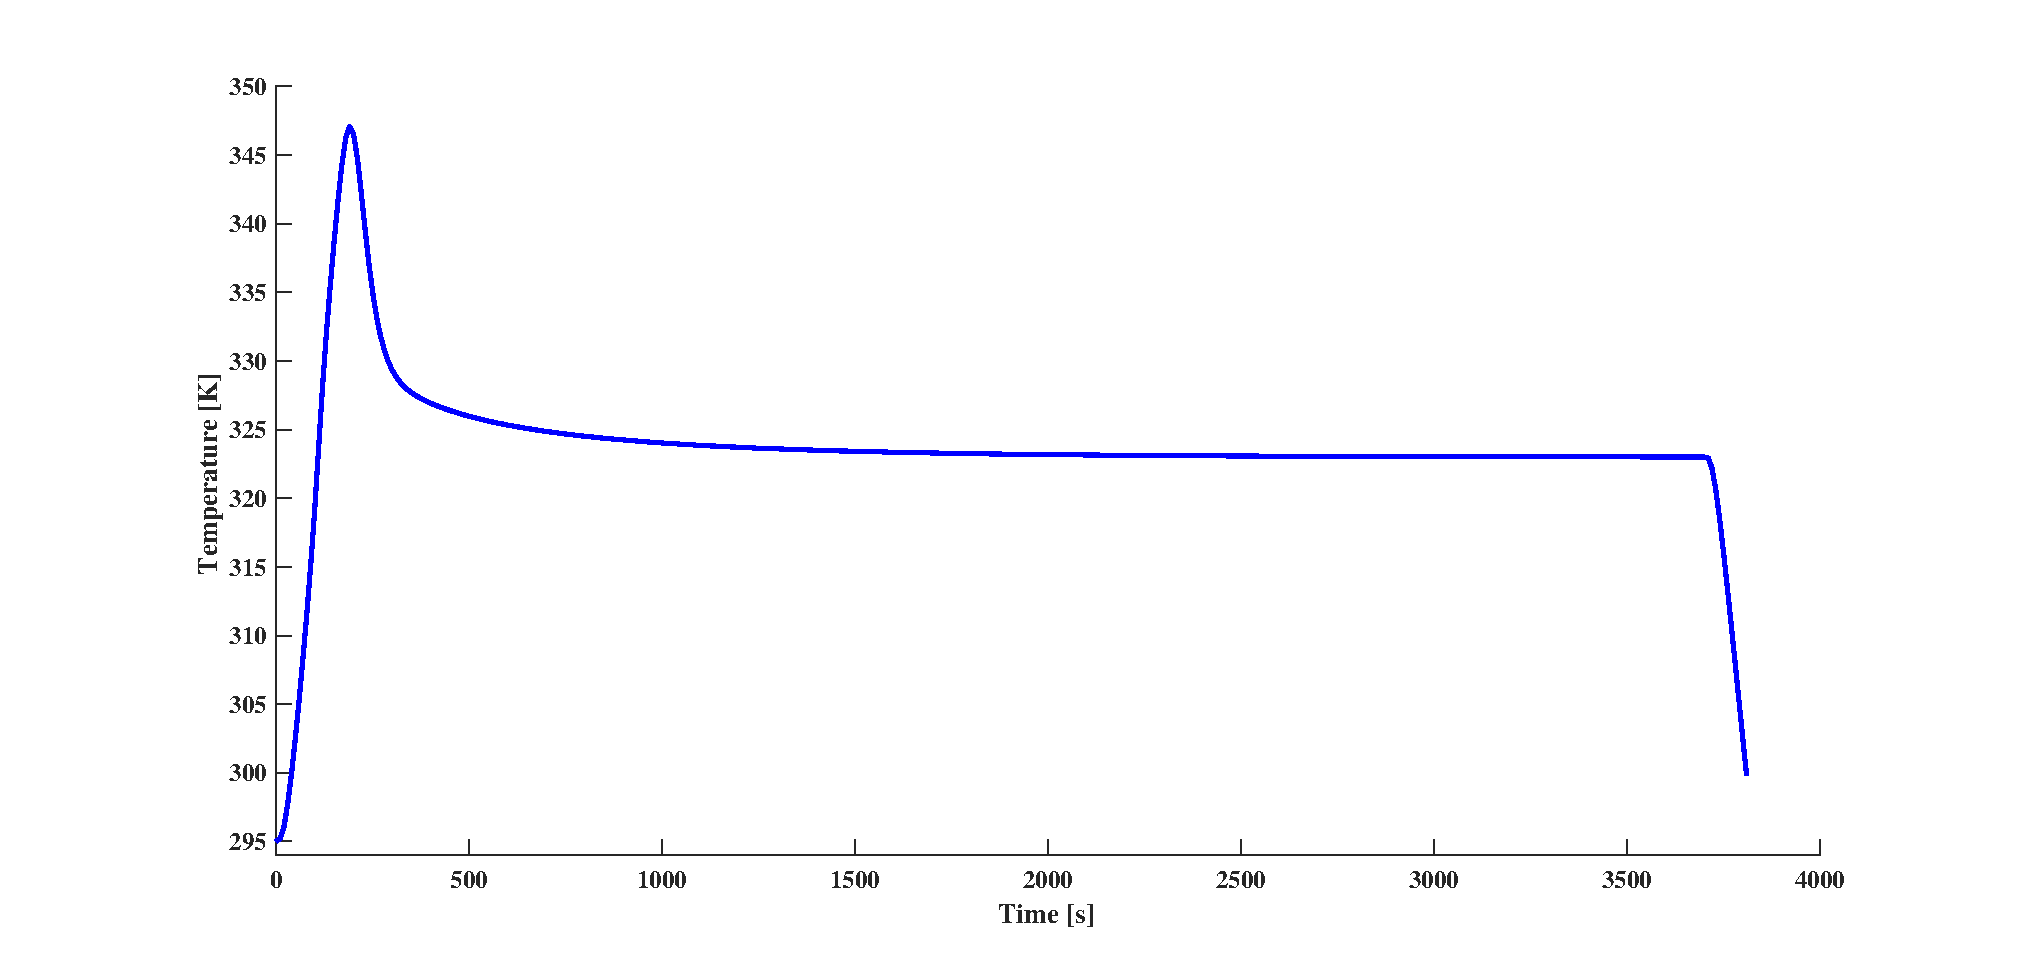
\includegraphics[width=0.9\textwidth]{obrazky/T-t.eps}
	\caption[Types of anchors]{Types of anchors ($h_{ef}$ is effective anchor length) \cite{anchors-ACI-318M}: a) cast-in-place; b) post-installed.}\label{obr:Curing_temperature}
\end{figure}

\begin{figure}[h!]
	\centering
	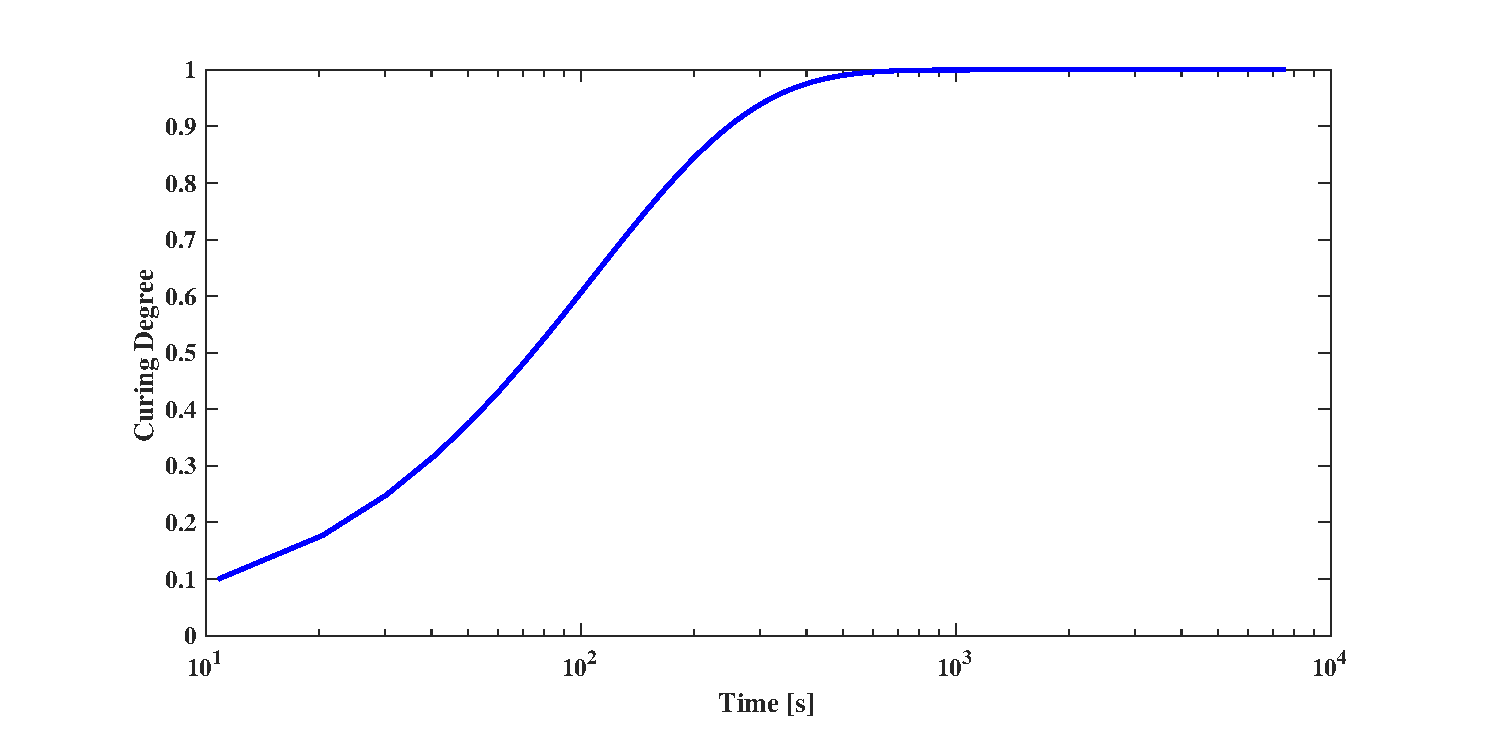
\includegraphics[width=0.9\textwidth]{obrazky/CD-t.eps}
	\caption[Types of anchors]{Types of anchors ($h_{ef}$ is effective anchor length) \cite{anchors-ACI-318M}: a) cast-in-place; b) post-installed.}\label{obr:Curing_curing}
\end{figure}


\cleardoublepage
\thispagestyle{plain}
\section*{Conclusion}
\addcontentsline{toc}{section}{\protect\numberline{}Conclusion}
\indent

%\thispagestyle{empty/plain/headings/myheadings}


\cleardoublepage
%\input{./kapitoly/kapitola7}

}
\setstretch{1.2}{
	\clearpage
	%\input{priloha0}
	\clearpage
	%\input{priloha1}
}


\cleardoublepage

\bibliography{thesisbiblio}


\begin{comment}
	Obsah...

\begin{thebibliography}{99}
	\bibitem{anchors-ACI-318M}
	ACI (2008). ACI 318M-08 Building code requirements for structural concrete. ACI
	
	\bibitem{hilti_anchors}
	Post-installed anchors. Hilti - mechanical vs adhesive anchors [online]. [cit. 2018-04-21].  
	
	Available from: $https$:$//ask.hilti.com/article/mechanical$-$vs$-$adhesive$-$anchors/rysrkl$
	
	\bibitem{adhesive_anchors}
	Sherief S.S. Sakla, Ashraf F. Ashour, \textit{Prediction of tensile capacity of single adhesive anchors using neural networks},	Computers $\&$ Structures \textbf{83} (2005) 1792-1803.
	
	\bibitem{thermosetting_polymers}
	PASCAULT, Jean-Pierre. Thermosetting polymers. New York: Marcel Dekker, c2002. Plastics engineering (Marcel Dekker, Inc.), 64. ISBN 08-247-0670-6.
	
	\bibitem{mars}
	More info on official site: 
	$http://mars.es3inc.com/www_es3inc_com/marssolver/$
	
	\bibitem{geofem}
	Prof. Ing. Michal Šejnoha, Ph.D., DSc. GEO FEM - Theoretical manual: A computer program for nonlinear finite element analysis of geotechnical problems. 2009, FINE Ltd. 1999-2009.
    	
\end{thebibliography}
\end{comment}
\end{document}
